\documentclass[a4paper,11pt, oneside]{article}  % document class
\usepackage{geometry}
\geometry{
  inner=20mm,
  outer=20mm,
  top=30mm,
  bottom=25mm %
%  heightrounded,
%  marginparwidth=50pt,
%  marginparsep=17pt,
%  headsep=20pt
}
\usepackage[english]{babel}
\usepackage{hyperref}
%pacchetto
\usepackage{import, multicol,lipsum}  % package
\setlength{\columnsep}{1cm}

\usepackage[utf8]{inputenc} % accenti facili
\usepackage[T1]{fontenc}
\usepackage{subcaption}
\usepackage{pifont}
\usepackage{url}
\hypersetup{
	colorlinks=true,
	linkcolor=blue,
	filecolor=magenta,      
	urlcolor=blue
}
\usepackage{graphicx, color, blindtext}
\usepackage{textcomp, makeidx, times}
\usepackage{amsthm, amsmath, amssymb, amsfonts, mathtools} % math
\usepackage[mathscr]{eucal}		
\usepackage[nottoc]{tocbibind} 
\usepackage{pgfplots, parskip}
\usepackage{afterpage, ifthen}
\usepackage{enumitem}
\pgfplotsset{compat=newest}
\usepackage{graphicx} % immagini
\graphicspath{ {image/} } % path cartella delle immagini
\usepackage{tikz} %graph
\usetikzlibrary{arrows,automata}
\usetikzlibrary{automata,arrows,positioning,calc,matrix}
\usepackage[linesnumbered,ruled,vlined]{algorithm2e}
\usepackage{booktabs}
\usepackage{colortbl}
\usepackage{siunitx}
\usepackage{tabularx, tabu}
\usepackage{relsize}
\usepackage{makecell, caption, chngcntr}
\usepackage{bbm}
\usepackage{diffcoeff}
\RequirePackage{fix-cm}


%
%____________________________________________________________________________________________________________________________
%____________________________________________________________________________________________________________________________
%____________________________________________________________________________________________________________________________
%____________________________________________________________________________________________________________________________
% INIZIO
\begin{document}

\setcounter{secnumdepth}{2}
\pagestyle{plain} % stile pagina (header, numerazioni)

\centerline {
\includegraphics[width=2cm]{logo.jpg}}
\begin{center}
Università degli Studi di Torino - M.Sc.  in Stochastic and Data Science - A.Y.  2021/2022 \\
\Large { Final project of Statistical Machine Learning (MAT0043)}
\line(1,0){450}\\ 
\vspace{0.4cm} 
{ \huge \textbf{Gene selection for cancer type classification} }
\vspace{0.1cm}
%\hspace{0cm} 
%Group: Bartoli Francesco,  Boetti Chiara (854411), Bordino Alberto (856592)
\line(1,0){450} \\
\end{center}

%____________________________________________________________________________________________________________________________
% ABSTRACT
In recent years, medicine has made a great step forward in finding new and efficient therapies for different diseases. Thanks to up-to-date technologies, collecting huge amount of data is no longer an issue, so that one can exploit them to define personalised treatments for patients. In particular, cancer genome scale screens are just one example of these applications. In particular, they provide valuable information about the role of genes in driving cancer growth. Thus, researches has developed a Cancer Dependency Map in order to identify genetic and pharmacologic dependencies. However, this is quite a challenging aim: the dataset is not at all easy to handle (high-dimensional, over than $\sim 17.000$ features) and the picked drug-targetable genes should only rely on a specific cancer type, thus imbalanced classes. \\
In this project, we apply cutting-edge Statistical Machine Learning algorithms to classify different cancer types and select the most relevant genes. After a quick exploratory analysis with PCA, we try Random Forest, Lasso-SVM and Neural Network classifiers and see how the same technique performs differently according to which tumour we are focusing on. In fact, our classification accuracies range from $45\%$ to $98\%$.  \textbf{Aggiungere altre conclusioni}
\medskip

\begin{multicols}{2}
\section{Introduction}
%The mutations that cause cancer cells to grow also confer specific vulnerabilities that normal cells lack. Some of these acquired alterations represent compelling therapeutic targets. The challenge is that, for the overwhelming majority of cancers, we do not fully understand the relationship between the genetic alterations of cancer and the dependencies they cause. To solve this problem, we are creating a “cancer dependency map” by systematically identifying genetic dependencies and small molecule sensitivities and discovering the biomarkers that predict them.
Scrivere che il cancro e' una malattia molto brutta e brevemente come funziona (aka le cellule impazziscono: svillupano mutazioni, diventano imprevedibile e causano problemi negli individui...). Il compito della medicina e' trovare delle cure (banana). E qua entra in gico DepMap: DNA arrays che raccolgono mutationi dei geni delle cellule cancerogene. \\
--------------- \\
Developing new cancer therapies is based on finding processes that selectively kill cancer cells. In particular, the Achilles project uses genome-wide screens to systematically identify essential genes and report vulnerabilities across hundreds of human cancers.

\section{Dataset}
We use two publicly available datasets, both found on the DepMap Portal website:
\begin{itemize}
	\item \textit{CRISPR\_gene\_dependency.csv}, which contains $1.032$ cancer cell lines characterised by $17.393$ gene scoring results; \\
	\item \textit{sample\_info.csv}, which contains cell lines information, such as primary disease and sample collection site.
\end{itemize}
Data were collected from real patients and successively processed, so that each element of this $(1.032 \times 17.393)$-matrix is the probability that knocking out a gene has a real depletion effect on the cell. \\
First of all, we look for any missing values: only 10 rows have empty columns, specifically either $678$ or $1.285$ Nas. At first impact, this could seem a big deal, but is actually the $4\%$ and $7\%$  of the total genes. Moreover, these cells come from different tumours, so we decide to simply remove them all.  \\
Before proceeding with our analysis, we also notice some weird observations: $2$ of them are labelled as "Non-Cancerous" and $6$ as "Engineered". The first can be reasonably discarded as our goal is classifying cancer cells, whereas the latter requires a little care. Engineered cells are synthetically modified sample in lab and, here, they are manly associated to the Eye sample collection site. We keep them and we associate the cancer type according to the sample. \\
One could ask: why do we focus only on the primary disease and not also on the sample collection site? If we count the number of cells with respect to cancer type and collections site, we find many peculiarities. For instance, some Brain-cancer cells have been picked from the abdomen, whereas Lung-cancer cells comes from a variety of different places. This is because of the nature/curse of cancer: metastasis are ill cells identifiable as the original tissue but found on a different site. Therefore, this subdivision would only complicate our task.  \\
Finally, we group the various cancer types in 10 classes according to common medical knowledge (\url{https://www.cancer.gov/types/by-body-location}) and we obtain the following classes:
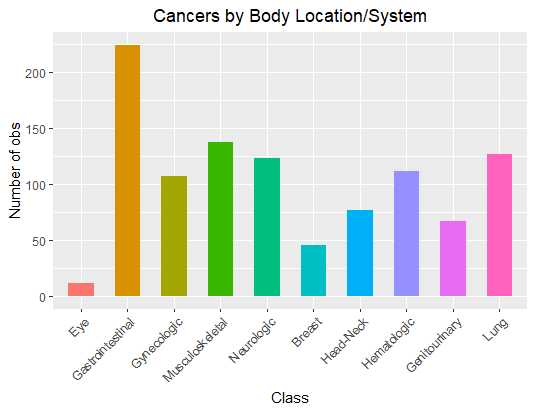
\includegraphics[width=9.5cm]{Rplot-classes.png}
\captionof{figure}{Cancer classes}\label{fig:a}

Figure \ref{fig:a} shows our classes.

\section{Methods}


\section{Results}



\section{Conclusion and future works}


\end{multicols}

\begin{thebibliography}{11}   % BIBLIOGRAFIA
% \bibitem{Baum} L. Baum, T. Petrie, \textit{Statistical Inference for Probabilistic Functions of Finite State Markov Chains}, in Ann. Math. Stat., 37, 1554-1563, 1966 \\
\bibitem{DepMap} DepMap Portal: \url{https://depmap.org/portal/}  \\
\bibitem{DepMapData} DepMap, Broad (2021): DepMap 21Q3 Public, figshare. Dataset: \url{https://doi.org/10.6084/m9.figshare.15160110.v2} \\
\bibitem{Achilles} Project Achilles: \url{https://depmap.org/portal/achilles/}  \\
\end{thebibliography}
\end{document}